%!TEX root = ../main.tex
\section{Different aspects of deep learning-based anomaly detection. }
\label{sec:aspectsOfAnomalyDetection}
This section identifies and discusses the different aspects of deep learning-based anomaly detection.

%%%%%%%%%%%%%%%%%%%%%%%% Begin of  Nature of Input data %%%%%%%%%%%%%%%%%%%%%%%%
\subsection{ Nature of Input Data}
The choice of deep neural network architecture in deep anomaly detection methods primarily depends on the nature of input data. Input data can be broadly classified into sequential (eg, voice, text, music, time series, protein sequences) or non-sequential data (eg, images, other data). Table~\ref{tab:dataTypeModelArchitecture} illustrates the nature of input data and deep model architectures used in anomaly detection. Additionally input data depending on the number of features (or attributes) can be further classified into either low or high-dimensional data. DAD techniques have been to learn complex hierarchical feature relations within high-dimensional raw input data ~\cite{lecun2015deep}. The number of layers used in DAD techniques is driven by the dimensionality of input data, deeper networks are shown to produce better performance on high dimensional data. Later on in the Section ~\ref{sec:deepDADModels}  various models considered for outlier detection are reviewed at depth.

%% Create a table with Type of data and kind of architecture suitable for anomaly detection.
\begin{table}
\centering
\begin{tabular}{ |c|c|c|c| }
\hline
Type of Data & Examples & DAD model architecture  \\ [0.5ex]
\hline
\multirow{3}{3em}{Sequential} & Video,Speech &  \\
&Protein Sequence,Time Series  & CNN, RNN, LSTM  \\
&Text (Natural language)  &  \\
\hline
\multirow{2}{3em}{Non-Sequential} & Image,Sensor &  \\
&Other (data)  & CNN, AE and its variants  \\
\hline
\end{tabular}
\caption{Table illustrating nature of input data and corresponding deep anomaly detection model architectures proposed in literature.
        \\CNN: Convolution Neural Networks, LSTM : Long Short Term Memory Networks \\
         AE: Autoencoders. }
\label{tab:dataTypeModelArchitecture}
\end{table}
% End of table
%%%%%%%%%%%%%%%%%%%%%%%% End of  Nature of Input data %%%%%%%%%%%%%%%%%%%%%%%%


%%%%%%%%%%%%%%%%%%%%%%%% Begin  Type of models %%%%%%%%%%%%%%%%%%%%%%%%
\subsection{Based on Availability of labels}
Labels indicate whether a chosen data instance is normal or outlier. Anomalies are rare entities hence it is very  difficult to obtain their labels. Furthermore anomalous behaviour may change over time, for instance  the nature of anomaly had changed so significantly and that it  remained unnoticed at Maroochy water treatment plant, for a long time which resulted in leakage of 150 million litres of untreated sewerage to local waterways ~\cite{ramotsoela2018survey}.\\
Deep anomaly detection (DAD) models can be categorized into three categories based on extent of availability of labels. (1) Supervised anomaly detection (SAD). (2) Semi-Supervised anomaly detection (SSAD). (3) Unsupervised anomaly detection (USAD).

\subsubsection{Supervised anomaly detection:}
\label{supervised_learning}
Supervised anomaly detection involves training a supervised binary or multi class classifier, using labels of both normal and anomalous data instances. Supervised DAD models, formulated as multiclass classifier in chapter IV of thesis, aids in identifying a legitimate drug name mention ~\cite{chalapathy2016investigation}.A supervised classifier trained on sequential text data used to identify a valid clinical concept~\cite{chalapathy2016bidirectional} is shown to produce state-of-the-art results.
Despite supervised methods are shown to perform well, supervised DAD methods are not as popular as semi-supervised or unsupervised methods owing to lack of availability of labeled training samples. Moreover the performance of supervised classifier used as anomaly detector is suboptimal due to class imbalance (the total number of positive class instances are far more than the total number of (negative) class of data). Therefore we do not consider the review of supervised DAD methods in this survey.


\subsubsection{Semi-supervised anomaly detection:}
\label{semi_supervised_learning}
The labels of normal instances are far more easy to obtain than anomalies, as a result semi-supervised DAD techniques are more widely adopted, these techniques leverage existing labels of single (normally positive class) to separate outliers. One common way of using deep autoencoders  in anomaly detection is to train them in a semi-supervised way on data samples with no anomalies. With sufficient training samples, of normal class autoencoders would produce low reconstruction errors for normal instances, over anomalous events.
~\cite{wulsin2010semi,nadeem2016semi,song2017hybrid}. We consider detailed review of these methods in  Section~\ref{sec:semi_supervised_DAD}.

%% Taxonomy of Models
%performance comparision
\begin{figure}[h]
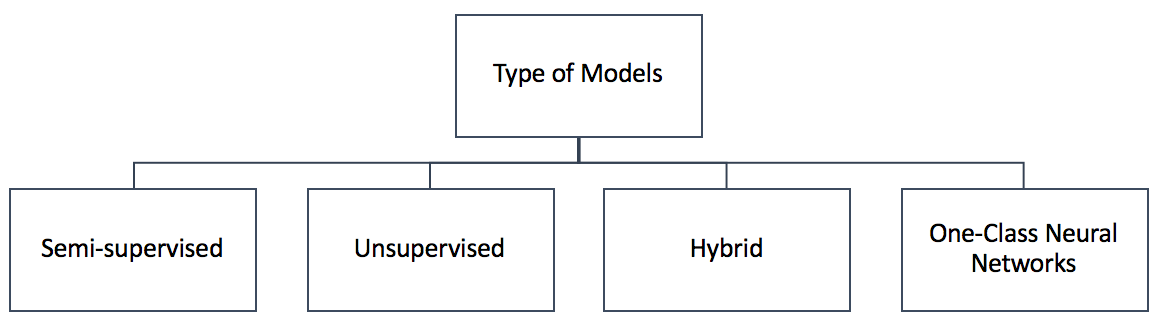
\includegraphics[scale=0.5]{images/TypeOfModels}
\captionsetup{justification=centering}
\caption{Taxonomy based on type of deep learning models for anomaly detection.}
\label{fig:typeOfModels}
\end{figure}

\subsubsection{Unsupervised anomaly detection (USAD):}
\label{sec:USAD}

Unsupervised anomaly detection techniques detect outliers solely based on intrinsic properties of the data instances. USAD techniques are used in automatic labelling of unlabelled data samplessince labeled data is very hard to obtain ~\cite{patterson2017deep}. Variants of USAD models~\cite{tuor2017deep} are shown to outperform traditional methods such as principal component analysis (PCA) ~\cite{wold1987principal}, support vector machine (SVM) ~\cite{cortes1995support} and Isolation Forest~\cite{liu2008isolation} techniques in applications domains such as health and cyber security.
Autoencoders are the core of all USAD models. These models assume the high prevalence of normal instances than abnormal data instances failing which would result in high false positive rate. Additionally unsupervised learning algorithms such as restricted Boltzmann machine (RBM)~\cite{sutskever2009recurrent}, deep Boltzmann machine (DBM), deep belief network (DBN)~\cite{salakhutdinov2010efficient}, generalized denoising autoencoders~\cite{vincent2008extracting} , recurrent neural network (RNN)~\cite{rodriguez1999recurrent} Long short term memory networks~\cite{lample2016neural} which are used to detect outliers are discussed in detail in Section ~\ref{sec:rnn_lstm_gru}.

\subsection{Based on training objective}
In this survey we introduce two new categories of deep anomaly detection (DAD) techniques based on training objective employed 1) Deep hybrid models (DHM). 2) One class neural networks (OC-NN).

\subsubsection{Deep Hybrid Models (DHM):}
\label{sec:DHM}

Deep hybrid models for anomaly detection use deep neural networks mainly autoencoders as feature extractors, the features learnt within the hidden representations of autoencoders are input to traditional anomaly detection algorithms such as one-class SVM (OC-SVM) to detect outliers~\cite{andrews2016detecting}. Figure~\ref{fig:HybridDeepModels} illustrates  the deep hybrid model architecture used for anomaly detection. Following the success of transfer learning to obtain rich representative features  from models pre-trained on large datasets,  hybrid models have also employed these pre-trained transfer learning models as feature extractors with great success ~\cite{pan2010survey}. A variant of hybrid model was proposed by  Ergen et.al~\cite{ergen2017unsupervised} which considers joint training of feature extractor alongwith OC-SVM (or SVDD) objective to maximize the detection performance. A notable shortcoming of these hybrid approaches
is the lack of trainable objective customised for anomaly detection, hence these models fail to extract rich differential features to detect outliers.  In order to overcome this limitation customised objective for anomaly detection such Deep one-class classification~\cite{ruff2018deep}and  One class neural networks~\cite{chalapathy2018anomaly} are introduced.

\begin{figure*}
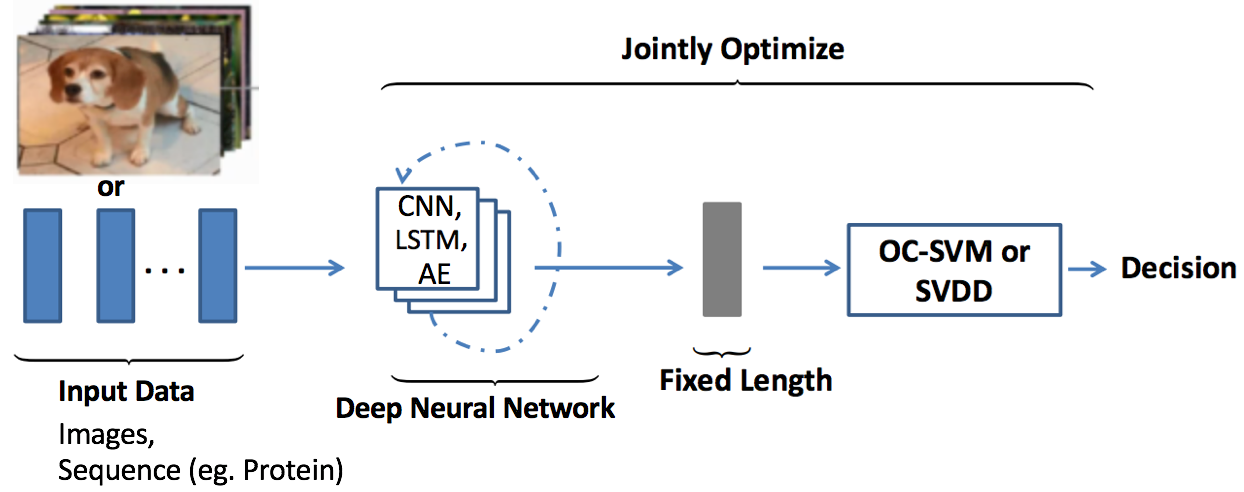
\includegraphics[scale=0.5]{images/HybridDeepModels}
\captionsetup{justification=centering}
\caption{Deep Hybrid Model Architecture.}
\label{fig:HybridDeepModels}
\end{figure*}

\subsubsection{One-Class Neural Networks (OC-NN):}
\label{sec:oc-nn}

One class neural network~\cite{chalapathy2018anomaly} methods are inspired by kernel-based one-class classification which combines the ability of deep networks to extract progressively rich representation of data with the one-class objective of creating a tight envelope around normal data. The OC-NN approach breaks new ground for the following crucial reason: data representation in the hidden layer is driven by the OC-NN objective and is thus customized for anomaly detection. This is a departure from other approaches which use a hybrid approach of learning deep features using an autoencoder and then feeding the features into a separate anomaly detection method like one-class SVM (OC-SVM).  The details of training and evaluation of one class neural networks is discussed in Section [XX] . Another variant of one class neural network architecture Deep Support Vector Data Description (Deep SVDD)~\cite{ruff2018deep} trains deep neural network to extract common factors of variation by closely mapping the normal data instances to the center of sphere, is shown to produce state-of-the-art results on MNIST and CIFAR-10 datasets.


%%%%%%%%%%%%%%%%%%%%%%%% End  Type of Models %%%%%%%%%%%%%%%%%%%%%%%%

\vspace{0.6cm}
\subsection{Type of Anomaly}
\label{sec:typeBasedAD}
Anomalies can be broadly  classified into three types: point anomalies, contextual anomalies and collective anomalies. Deep anomaly detection (DAD) methods have been shown to detect all three types of anomalies with great success.

% classification tree
\begin{figure}[h]
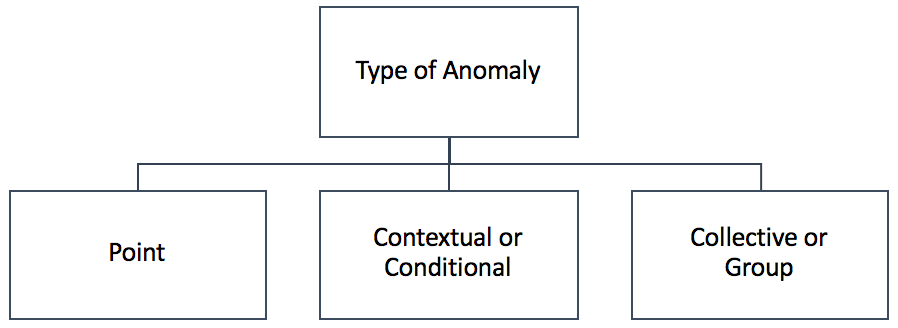
\includegraphics[scale=0.5]{images/TypeOfAnomaly}
\captionsetup{justification=centering}
\caption{Deep learning techniques classification based on type of anomaly.}
\label{fig:typeOfAnomaly}
\end{figure}


% Point Anomaly
\subsubsection{Point Anomalies.}
The majority of work in literature focuses on point anomalies. Point anomalies often represent an irregularity or deviation that happens randomly and may have no particular interpretation. For instance in Figure~\ref{fig:PointAndCollectiveAnomaly} a credit card transaction with high expenditure recorded at
\textit{Monaco} restaurant seems a point anomaly since it significantly deviates from the rest of the transactions. Several real world applications, considering point anomaly detection are reviewed in Section~\ref{sec:applicationsOfDLAD}.

% Contextual Anomaly
\subsubsection{Contextual Anomaly Detection.}
\label{sec:contextualanomalies}
Contextual anomaly also referred as conditional anomaly is a data instance that could be considered as anomalous in some specific context~\cite{song2007conditional}. The contextual anomaly is identified by considering both contextual and behavioural features.
The contextual features, normally used are time and space. While the behavioral features may be pattern of spending money, occurence of system log events, or any feature used to describe the normal behaviour.
Figure ~\ref{fig:temperatureContextual} illustrates the example of contextual anomaly considering temperature data indicated by a drastic drop just before June, this value is not indicative of a normal value found during this time. Figure ~\ref{fig:deeplogContextual} illustrates using deep Long Short-Term Memory (LSTM)~\cite{hochreiter1997long}  based model to identify anomalous system log events ~\cite{du2017deeplog} in a given context.

% Begin of figure
\begin{figure}
  \centering
  \begin{minipage}{.48\linewidth}
    \centering
    % \subcaptionbox{}
      {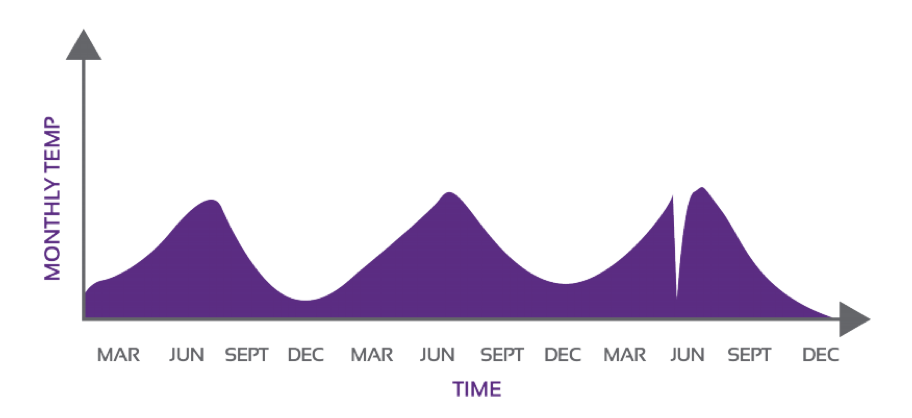
\includegraphics[scale=0.35]{images/temperature.png}}
    \caption{Illustration of contextual anomaly detection in two-dimensional temperature data set.}
    \label{fig:temperatureContextual}
  \end{minipage}\quad
  \begin{minipage}{.48\linewidth}
    \centering
    % \subcaptionbox{t}
      {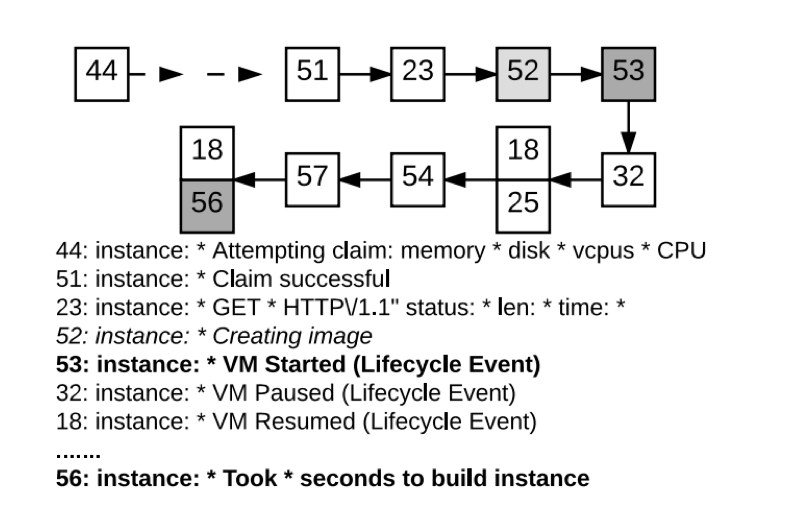
\includegraphics[scale=0.35]{images/deeplog.png}}
    \caption{Illustration of contextual anomaly detection in system logs.}
    \label{fig:deeplogContextual}
  \end{minipage}
  \bigskip

\end{figure}
% end of figure


% classification tree
% \begin{figure}[h]
% 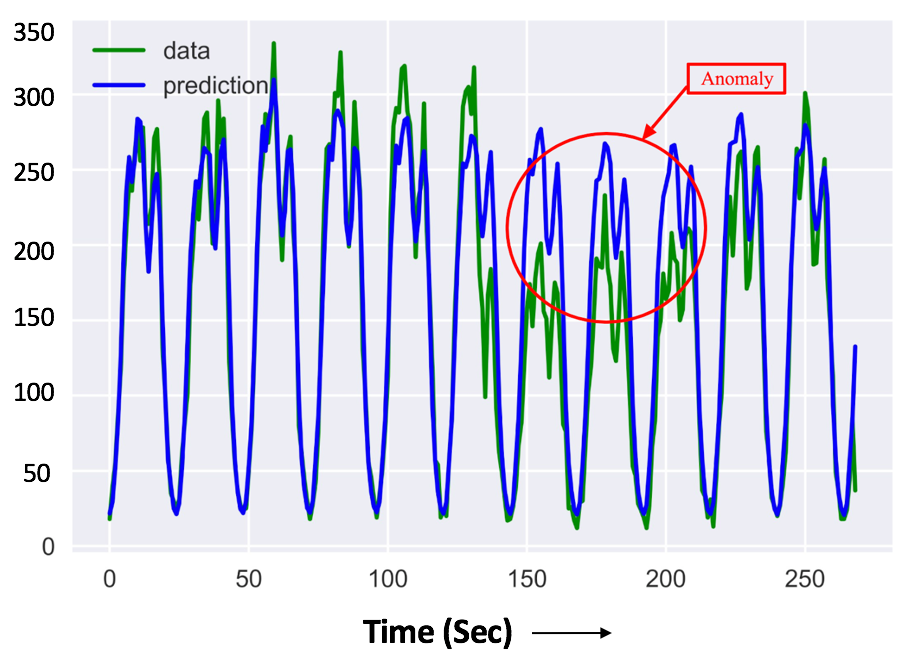
\includegraphics[scale=0.5]{images/ContextualAnomaly}
% \captionsetup{justification=centering}
% \caption{Predicted Vs Actual Data : Illustrating Contextual Anomaly.}
% \label{fig:ContextualAnomaly}
% \end{figure}


% Collective or Group Anomaly detection
\subsubsection{Collective or Group Anomaly Detection.}
Anomalous collections of individual data points are known as collective or group anomalies, wherein each of the individual points in isolation appear as normal data instances while observed in a group exhibit unusual characteristics. For example, consider an illustration of fraudulent credit card transaction, in the log data shown in Figure~\ref{fig:PointAndCollectiveAnomaly}, if a single transaction of "MISC" would have occured, it might probably not seem as anomalous. The consecutive group of transactions of valued at $\$75$ certainly seems to be a candidate for collective or group anomaly.
Group anomaly detection (GAD) with an emphasis on irregular group distributions (e.g. irregular mixtures of image pixels are detected using a variant of autoencoder model~\cite{chalapathy2018group,bontemps2016collective,araya2016collective,zhuang2017group}
% classification tree
\begin{figure}[h]
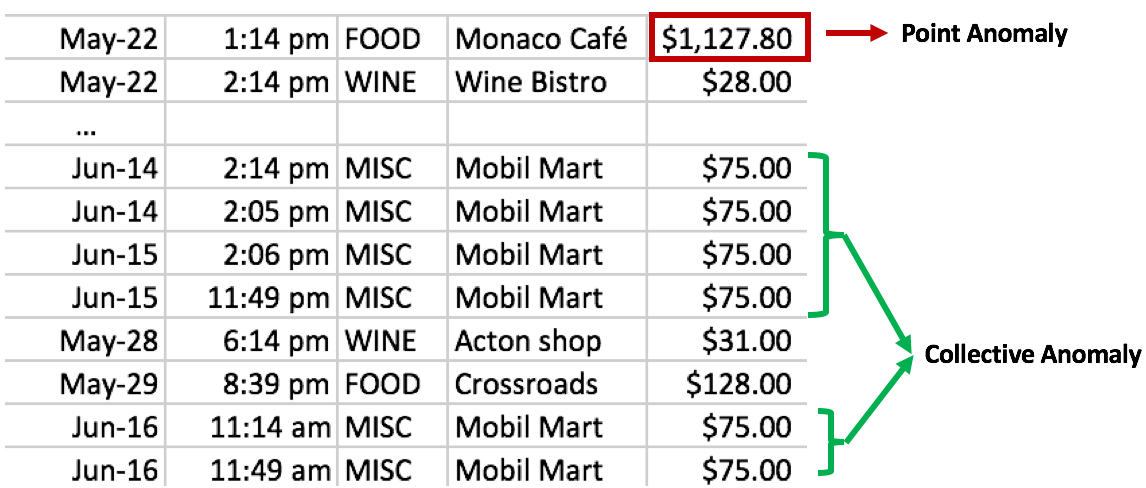
\includegraphics[scale=0.5]{images/PointAndCollectiveAnomaly}
\captionsetup{justification=centering}
\caption{Credit Card Fraud Detection: Illustrating Point and Collective anomaly.}
\label{fig:PointAndCollectiveAnomaly}
\end{figure}
%%%%%%%%%%%%%%%%%%%%%%%% End  Type of Anomalies %%%%%%%%%%%%%%%%%%%%%%%%


% Collective anomaly is also known as  group anomaly. While each individual data instances of this group may not be an anomaly, but their occurrence together as a collection is anomalous.

% Output of deep learning based anomaly detection methods
\subsection {Output of DAD Techniques}
\label{output_of_dad_methods}
An critical aspect for anomaly detection methods is the way in which the anomalies are identified. Generally, the outputs produced by anomaly detection methods are either anomaly score or binary labels.

\subsubsection{Anomaly Score:}
 Anomaly score describes the level of \textit{outlierness} for  each datapoint. The data instances may be ranked according to  anomalous score, and a domain specific threshold (commonly known as decision score) will be selected by subject matter expert to identify the anomalies.  In general, decision scores reveal more information than binary labels. In Deep SVDD approach the decision score is the measure of distance of data point from center of the sphere, the data points which are farther away from center are considered anomalous.

\subsubsection{Labels:} Instead of assigning scores, some techniques may assign a category label as normal or anomalous to each data instance. Unsupervised anomaly detection techniques using autoencoders measure  the magnitude of residual vector (i,e reconstruction error) for obtaining anomaly scores, later on the reconstruction errors are either ranked or thresholded by domain experts to label data instances.
%%%%%%%%%%%%%%%%%%%%%%%% End  Output of deep learning based AD %%%%%%%%%%%%%%%%%%%%%%%%

